\documentclass{oblivoir}
\usepackage{amsmath,amssymb,amsthm,kotex,mdframed,paralist,graphicx,tabu}
\newcommand\pb[1]{\ensuremath{\fbox{\phantom{#1}}}}

\usepackage{fapapersize}
\usefapapersize{210mm,297mm,40mm,40mm,30mm,30mm}

\newcounter{num}
\newcommand\prob[1]
{\bigskip\par\noindent\stepcounter{num} \textbf{문제 \thenum) #1}\par\noindent}
\newcommand\ans[1]
{\par{\raggedleft\textbf{답 : #1}
\par}\bigskip\bigskip}
%%%
\begin{document}

%%%
\section{다항식의 연산}
%%
\subsection{다항식의 연산법칙}
\begin{align*}
&A+B=B+A 			\tag{덧셈의 교환법칙}\\
&AB=BA 				\tag{곱셈의 교환법칙}\\
&(A+B)+C=A+(B+C)	\tag{덧셈의 결합법칙}\\
&(AB)C=A(BC)		\tag{곱셈의 결합법칙}\\
&A(B+C)=AB+AC		\tag{분배법칙}
\end{align*}

%%
\subsection{다항식의 나눗셈과 정수의 나눗셈}
다항식 \(A\)를 \(B\)로 나누었을 때의 몫을 \(Q\), 나머지를 \(R\)이라고 하면
\[A=BQ+R\quad(\text{단, }B\text{의 차수}>R\text{의 차수})\]

\noindent
정수 \(a\)를 자연수 \(b\)로 나누었을 떄의 몫을 \(q\), 나머지를 \(r\)이라고 하면
\[a=bq+r\quad(0\le r<b)\]


%%
\subsection{나머지정리와 인수정리}
나머지정리 : 다항식 \(f(x)\)를 \(x-\alpha\)로 나눈 나머지는 \(f(\alpha)\)이다.\\
인수정리 : \(P(\alpha)=0\iff P(x)\)가 \(x-\alpha\)로 나누어 떨어진다.

%%
\subsection{인수분해}
\begin{enumerate}
\item[①]
공통인수로 묶어본다.
\item[②]
인수분해 공식을 사용한다.
\begin{align*}
a^3+b^3+c^3-3abc
&=(a+b+c)(\pb{\(a^2+b^2+c^2-ab-bc-ca\)})\\
&=(a+b+c)\left[\frac12\left\{\pb{\((a-b)^2+(b-c)^2+(c-a)^2\)}\right\}\right]\\
a^4+a^2b^2+b^4&=\pb{\((a^2+ab+b^2)\)})(\pb{\((a^2-ab+b^2)\)}\\
x^7-1&=(x-1)(\pb{\(x^6+x^5+x^4+x^3+x^2+x+1\)})
\end{align*}
\item[③]
치환/조립제법/계수가 대칭인 사차식
\[x^4-4x^3+5x^2-4x+1=(\pb{\(x^2-x+1\)})(\pb{\(x^2-3x+1\)})\]
\item[④]
한 문자에 대해 내림차순으로 정리
\[a^2(b-c)+b^2(c-a)+c^2(a-b)=\pb{\(-(a-b)(b-c)(c-a)\)}\]
\end{enumerate}

\newpage
%%%
\section{방정식과 부등식}

%%
\subsection{복소수}
\begin{enumerate}[(1)]
\item
\(i^2=-1\)
\item
\(i^{4k}=\pb1\), \(i^{4k+1}=\pb i\), \(i^{4k+2}=\pb{-1}\), \(i^{4k+3}=\pb{-i}\)
\item
\(\sqrt{-3}=\pb{\(\sqrt3\)}i\)
\item
\(\sqrt a\sqrt b=\begin{cases}
 \sqrt{ab}&(\text{otherwise})\\
-\sqrt{ab}&(a<0, b<0)
\end{cases}\)
\\
\(\frac{\sqrt a}{\sqrt b}=\begin{cases}
 \sqrt{\frac ab}&(\text{otherwise})\\
-\sqrt{\frac ab}&(\pb{a<0, b<0})
\end{cases}\)
\item
\(z=a+bi\)이면, \(z+\bar z=\pb{2a}\), \(z\bar z=\pb{\(a^2+b^2\)}\)
\item
\(\bar z=z\iff z\)는 실수
\item
\(\overline{z+w}=\bar z+\bar w\), \(\overline{zw}=\bar z\bar w\)
\item
\(1+2i\)가 방정식 \(x^3-4x^2+9x-10=0\)의 근이면 \pb{\(1-2i\)}도 이 방정식의 근이다.
\end{enumerate}

%%
\subsection{이차방정식과 이차함수, 이차부등식}
\noindent
{\footnotesize
\begin{tabular}{p{0.24\textwidth}|p{0.24\textwidth}|p{0.24\textwidth}|p{0.24\textwidth}}
\hline
&\qquad\qquad\(D>0\)		&\qquad\qquad\(D=0\)	&\qquad\qquad\(D<0\)\\
\hline
\(y=ax^2+bx+c\)의 그래프
&\raisebox{-.5\height}{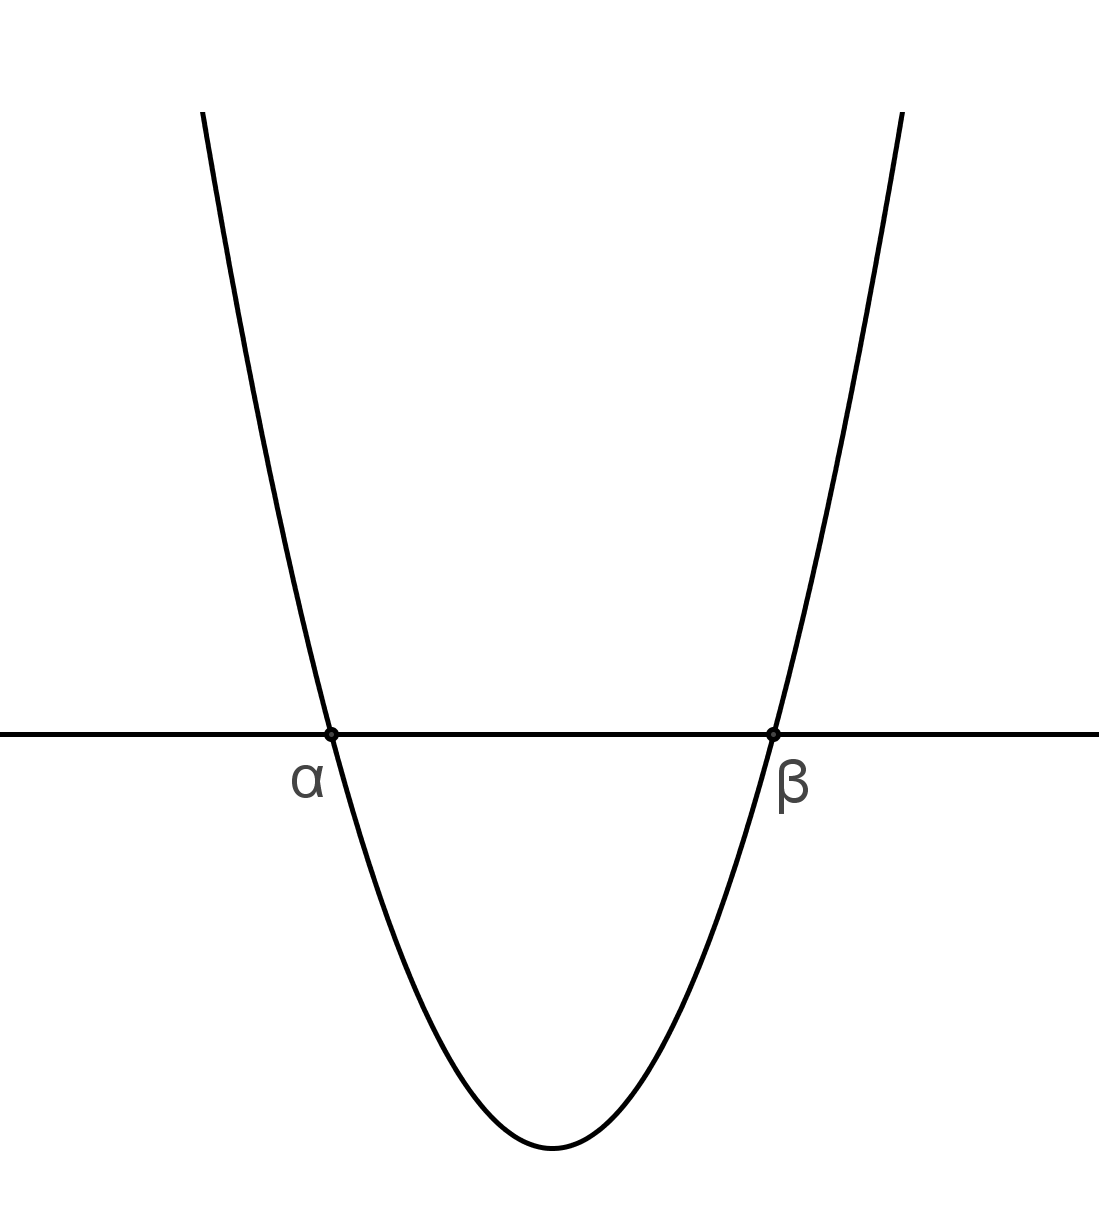
\includegraphics[width=0.24\textwidth]{1}}
&\raisebox{-.5\height}{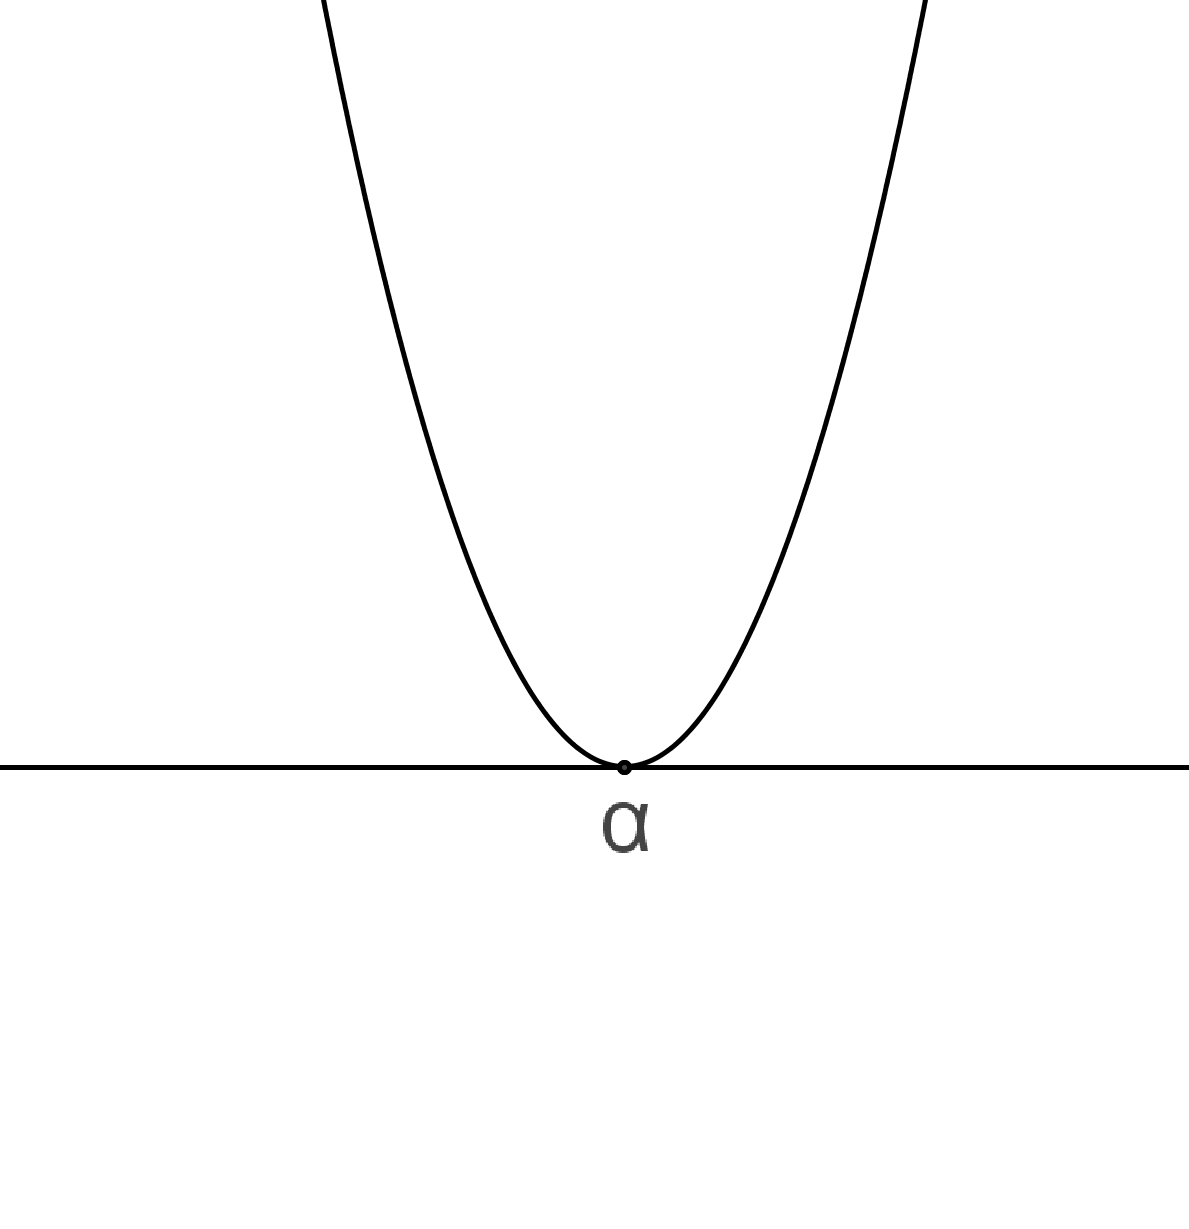
\includegraphics[width=0.24\textwidth]{2}}
&\raisebox{-.5\height}{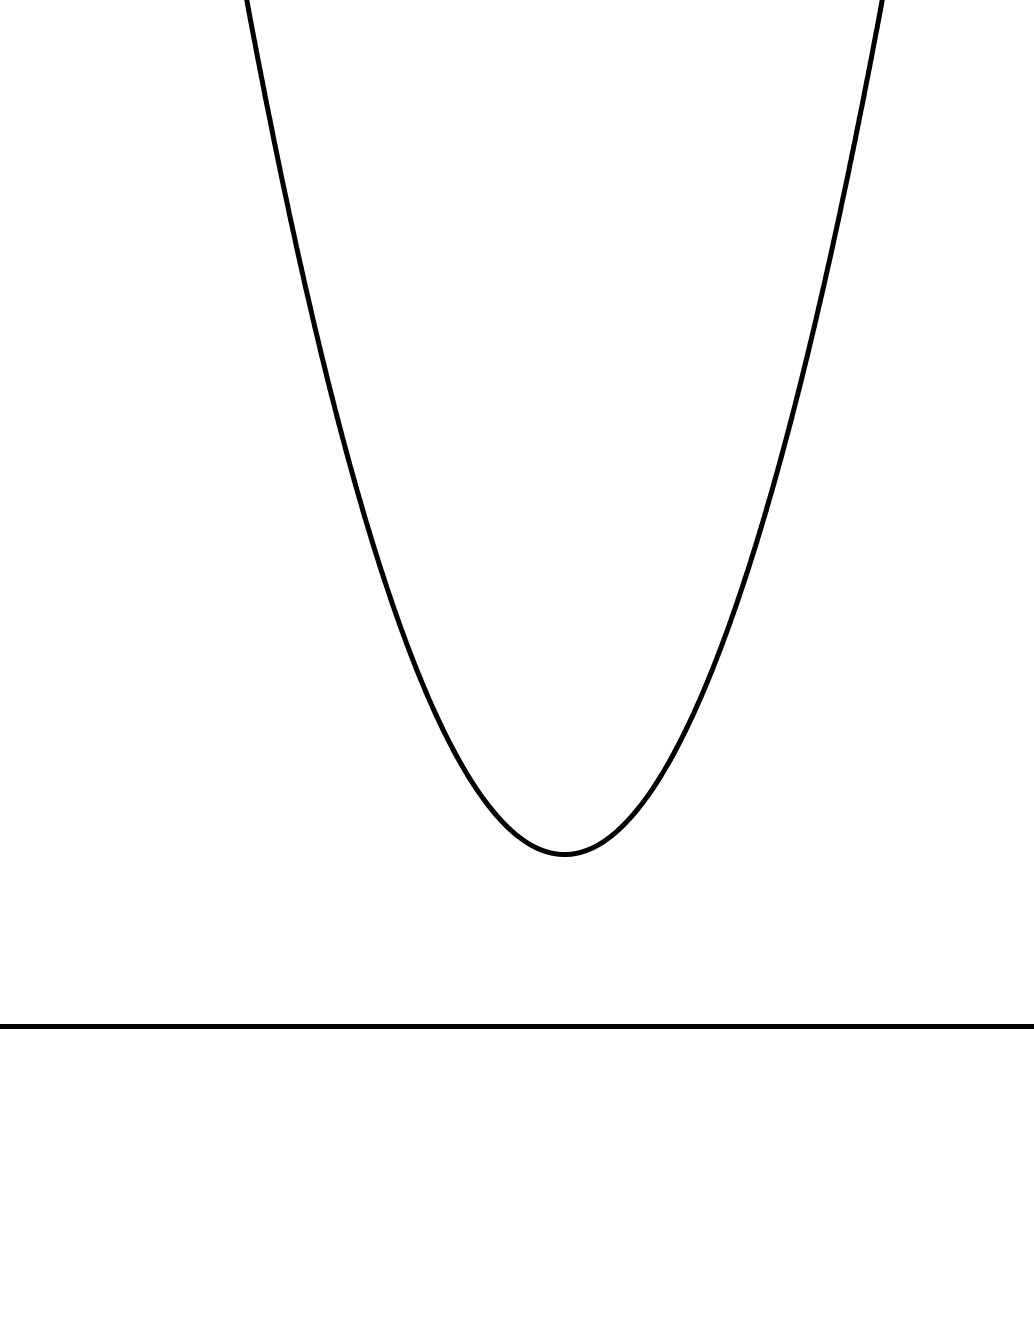
\includegraphics[width=0.24\textwidth]{3}}\\\hline
\(ax^2+bx+c=0\)의 해
&\(x=\alpha\) 또는 \(x=\beta\)		&\(x=\alpha\)	&근이 없다\\\hline
\(ax^2+bx+c>0\)의 해
&\(x<\alpha\) 또는 \(x>\beta\)		&\(x\neq\alpha\)인 모든 실수	&모든 실수\\\hline
\(ax^2+bx+c\ge0\)의 해
&\(x\le\alpha\) 또는 \(x\ge\beta\)	&모든 실수					&모든 실수\\\hline
\(ax^2+bx+c<0\)의 해
&\(\alpha<x<\beta\)				&없다.					&없다.\\\hline
\(ax^2+bx+c\le0\)의 해
&\(\alpha\le x\le\beta\)			&\(x=\alpha\)				&없다.\\\hline
\end{tabular}
}

%%
\subsection{\(1\)과 \(-1\)의 세제곱근, \(\omega\)}
\begin{minipage}{0.49\textwidth}
\(x^3=1\)의 한 허근을 \(\omega\)라고 하면
\begin{enumerate}
\item[①]
\(\omega^3=1\)
\item[②]
\(\omega^2+\omega+1=0\)
\item[③]
\(\omega+\bar\omega=-1,\quad\omega+\bar\omega=1\)
\end{enumerate}
\end{minipage}
\begin{minipage}{0.49\textwidth}
\noindent
\(x^3=-1\)의 한 허근을 \(\omega\)라고 하면
\begin{enumerate}
\item[①]
\(\omega^3=-1\)
\item[②]
\(\omega^2-\omega+1=0\)
\item[③]
\(\omega+\bar\omega=1,\quad\omega+\bar\omega=1\)
\end{enumerate}
\end{minipage}

\newpage
%%%
\section{문제들}
%
\prob{}
다항식 \(P(x)=x^3+ax^2+bx+2\)가 \((x-1)^2\)으로 나누어떨어질 때, 상수 \(a\), \(b\)에 대하여 \(a^2+b^2\)의 값을 구하여라.
\ans{\(9\)}

%
\prob{}
다항식 \(f(x)\)를 \((x-1)^2\)으로 나누었을 때의 나머지는 \(x+2\)이고, \(x-2\)로 나누었을 떄의 나머지는 \(3\)이다.
\(f(x)\)를 \((x-1)^2(x-2)\)로 나누었을 때의 나머지는?
\ans{\(-x^2+3x+1\)}

%
\prob{}
\(2^{1001}\)을 \(15\)로 나누었을 때의 나머지는?
\ans{\(2\)}

%
\prob{}
\(x^2-4xy+ky^2+6x-8y+5\)가 두 일차식의 곱으로 인수분해될 때, 실수 \(k\)의 값은?
\ans{\(3\)}

%
\prob{}
이차방정식 \(f(x)=0\)의 두 근을 \(\alpha\), \(\beta\)라고 하면 \(\alpha+\beta=6\)이다.
이때 이차방정식 \(f(4x-3)=0\)의 두 근의 합은?
\ans{\(3\)}

%
\prob{}
이차방정식 \(x^2-4x+k+1=0\)의 두 근이 모두 양수가 되도록 하는 실수 \(k\)의 값의 범위를 구하여라.
\ans{\(-1<k\le3\)}

%
\prob{}
\(-1\le x\le2\)일 때, 함수
\[y=(x^2-2x+3)^2-2(x^2-2x+3)-4\]
의 최댓값과 최솟값의 합은?
\ans{\(16\)}

%
\prob{}
방정식 \(x^3=-1\)의 한 허근을 \(\omega\)라고 할 때, \(\frac{\omega-1}{\omega^2}+\frac{\omega^2}{\omega-1}\)의 값을 구하여라.
\ans{\(2\)}

%
\prob{}
다음 연립방정식을 만족시키는 \(x\), \(y\)에 대하여 \(x^2+y^2\)의 최댓값을 구하여라.
\[\begin{cases}
x^2-xy-2y^2=0\\
2x^2+y^2=9
\end{cases}\]
\ans{\(6\)}

%
\prob{}
다음 연립방정식을 만족시키는 \(x\), \(y\)에 대하여 \(x^2+y^2\)의 최댓값을 구하여라.
\[\begin{cases}
x^2-xy=2\\
2xy-y^2=3
\end{cases}\]
\ans{\(5\)}

%
\prob{}
다음 연립방정식을 만족시키는 \(x\), \(y\)에 대하여 \(x^2+y^2\)의 최댓값을 구하여라.
\[\begin{cases}
x^2+y^2+x+y=4\\
x^2+xy+y^2=3
\end{cases}\]
\ans{\(5\)}

%
\prob{}
이차방정식 \(x^2-(a-3)x+a-2=0\)의 두 근이 모두 정수일 때, 상수 \(a\)의 값의 합을 구하여라.
\ans{\(10\)}

\end{document}